\section{Battery selection}
\label{Chap:Battery_Selection}
In the current Solar Jet project, the Schübeler 7800 HDME battery has been chosen as the energy carrier unit. A detailed argumentation is lacking however. In this section therefore it is investigated what the battery requirements are for the set goal of the project. A battery selection process will then finally decide upon a suitable battery.
\subsection{Requirements}
\begin{enumerate}
\item Energy\\
The Solar Jet project's short term goal is to set a speed of 450\textit{km/u}. In a previous bachelor thesis of Jasper Oranje \cite{BEP_Jasper} it is noted that this speed is only achievable for a short amount of time because of the EDF heating up. For the energy required, it is then assumed that the Solar Jet has to be able to fly at a cruising speed of 394\textit{km/u} for up to three minutes. With an energy transmission efficiency of 0.7, it is now calculated that the battery needs 547.22\textit{Wh}. This only accounts for overcoming the drag force, and does not take into account the energy needed for acceleration.\\
For the EDF to thrust full power, it draws around 9000\textit{W} and requires a voltage of approximately 50\textit{V}. The current draw can now be calculated from equation \ref{Eq:current_draw}.
\begin{equation}
\label{Eq:current_draw}
I = \frac{P}{V} = \frac{9000}{50} = 180 \textit{A}
\end{equation}
Now the voltage, the current and the capacity needed for a three minute cruise flight are determined.
\item Safety\\
Lithium-ion batteries are vulnerable to safety issues and can violently decompose when these are not met. The battery should therefore never exceed safety margins set by the manufacturer, which usually include a thermal operating range, a voltage operating range and a maximal charge and discharge current as described in section \ref{Chap:Battery_Safety}.\\
Furthermore the battery should be able to handle crashes. Especially with pouch cells, a construction has to be created to handle mechanical impact preventing internal short-circuit, since a hard-metal casing is non-present.
\item Other\\
Lastly, there are three more aspects. The battery should be as light as possible, as every addition of weight requires more thrust to accelerate. Besides weight, the battery should be dimensioned proportionally so that it fits in the allocated design space. Finally, the battery must be practical: The battery has to be easily removable from the Solar Jet for charging or inspection. The battery assembly from the individual cells must be manageable as well.
\end{enumerate}
\subsubsection{Cylindrical versus Pouch cells}
The first decision to make is whether to use cylindrical cells or pouch cells. Cylindrical cells come with safety, but also come with complexity, weight and volume. Pouch cells on the other hand come with energy density and relative simplicity, but might be prone to failure.

\textit{Cylindrical cell battery pack}\\
Cylindrical lithium-ion cells come in several sizes, but the 18650 size is almost exclusively used. 18650 stands for 18\textit{mm} in diameter, and 650\textit{mm} in length. Since the size is standardized, the range of options shrinks dramatically. There is only a few select creditable manufacturers and only a few select of chemistries to choose from. To further decrease this list of viable options, the influence of energy requirements has to be checked. 18650 cells always have a nominal voltage of 3.6 or 3.7\textit{V}. This means 14 battery packages in series for the required 50\textit{V} voltage. For the current, 180\textit{A} is needed for the EDF. 18650 batteries can not handle currents of 180\textit{A}, and thus need to be placed in parallel. The amount of batteries in parallel depends on the maximal current one cell is able to handle. In table \ref{Table:18650_cell_comparison} four option are listed. Battery info comes from Batterybro \cite{Batterybro}, a 18650 cell vendor that sells top brand batteries, includes the manufacturers spreadsheet and rates batteries themselves as well to correct for 'enthusiastic' spreadsheets.
\begin{table}[H]
\centering
\caption{18650 cell package needed for 50\textit{V}, 180\textit{A}}
\label{Table:18650_cell_comparison}
\begin{tabular}{|l|l|l|l|l|l|l|}
\hline
Battery & Cur.(\textit{A}) & Cap.(\textit{Ah}) & Pack & Total cap.(\textit{Wh}) & Weight(\textit{kg}) & Cost(\textit{\euro})* \\
\hline\hline
Sony VTC4			& 30			& 2							& 14S6P  & 604.8 & 3.780 & 281.40\\ \hline
LG Chem HB6			& 30				& 1.5				    & 14S6P & 453.6 & 4.032 & 205.80	 \\ \hline
Samsung INR-25R5			& 20			& 2.5			    & 14S9P & 1134.0 & 5.670 &565.74\\ \hline\hline
Panasonic NCR-B			& 5			& 3.4			    & 14S6P & 1056.8 & 3.780 & 335.16\\ \hline
\end{tabular}
\end{table} 
* Prices from \cite{Nkon}\\
\newline
The table lists the highest current batteries for all four major 18650 manufacturers. It can be seen that the Sony VTC4 would be the best choice for the Solar Jet its requirements. Because of the high current it is able to safely handle, only six cells have to be placed in parallel, drastically diminishing the total cell count compared to the Samsung INR battery. The battery would also suffice the total capacity needed for a three minute flight. The Samsung INR needs more batteries, and additionally has more capacity per battery. This makes for high capacity battery pack. This amount of capacity is however not needed and is a source of additional weight, making it a poor choice. The LG Chem is an overall worse choice than the Sony VTC4. Lastly the Panasonic is added to the list. For the Solar Jet a 14S36P package would be required. This would be over 22\textit{kg} and is not feasible. If a 14S6P pack is created out of Panasonics, it can be noted that the same weight and number of batteries have more capacity, but offers only 30\textit{A}. Because of this, this battery is used by Tesla as their energy carrier. It is added to this list to show that it is important to choose a battery specifically for requirements set by a project, as the Tesla cars apparently need more capacity than power, whereas the Solar Jet needs more power than capacity.
\begin{figure}[H]
  \centering
  \subfloat[Glued battery pack (13S14P).]{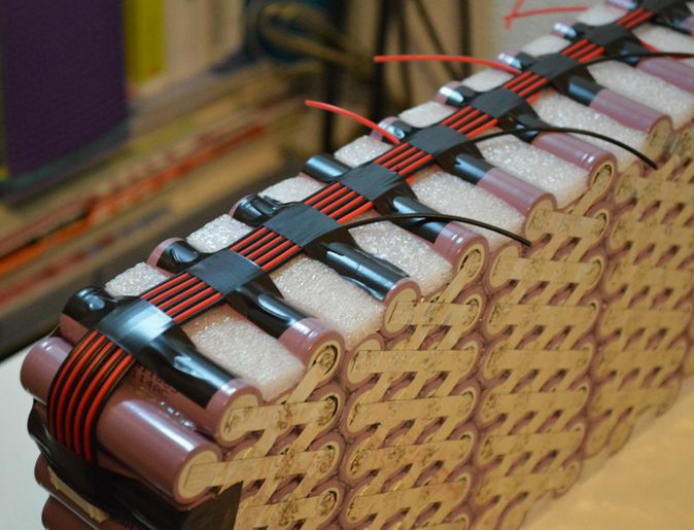
\includegraphics[width=0.5\textwidth]{Figures/BatteryDIY11.png}\label{Fig:18650_glued}}
  \hfill
  \subfloat[Spacer battery pack (7S5P)]{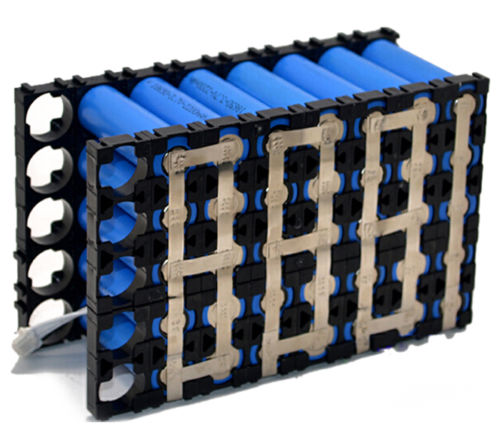
\includegraphics[width=0.5\textwidth]{Figures/batterypack.jpeg}\label{Fig:18650_spacer}}
  \caption{18650 Battery packs.}
  \label{Fig:18650_battery_packs}
\end{figure}
\textit{Building an 18650 battery pack}\\
Building a battery pack for the Solar Jet with 18650 batteries is tedious. Two different approaches are given in figure \ref{Fig:18650_battery_packs}. Creating such packs requires three steps:
\begin{enumerate}
\item Grouping\\
All parallel batteries have to be first grouped and attached to each other. This can be done by either gluing the batteries to each other like in figure \ref{Fig:18650_glued}, or using individual 3D printed spacers that make up an array like in figure \ref{Fig:18650_spacer}. A parallel group can then be connected to the next parallel group making a series connection. It is of course possible to make several parallel groups, spread them throughout the Solar Jet, and then connect all parallel groups in series via cables.
\item Connecting\\
Connecting batteries to each other is done via soldering or preferably spot welding metallic strips in between batteries. Spot welding here is better because soldering will transfer more heat to the battery than spot welding the strips. A parallel connection connects either a positive to positive, or a negative to negative terminal, whereas for series connection a negative terminal connects to a positive terminal (or in reverse).
\item Finishing\\
Finally cables have to be soldered onto the end terminals for the (dis)charge circuit. These cables need to be able to handle the total current and voltage output of the battery pack. Smaller cables (seen in figure \ref{Fig:18650_glued}) need to be soldered onto all end terminals of each individual parallel group. This forms the balancing circuit as explained in section \ref{Chap:Battery_Safety}. During discharge, a battery management system can be attached to this balancing circuit as well to monitor each individual parallel group voltage. Finally a heat shrink can be added to cover everything neatly.
\end{enumerate}
Building an 18650 battery pack is complex, especially for the Solar Jet project with 86 batteries to weld and solder strips and wires to. This requires a lot of effort to do right. A further disadvantage of an 18650 battery pack is that balancing and battery monitoring can only happen for each in series connected group. For the Solar Jet this would mean all 14 6P groups can be monitored individually, but those six cells connected in parallel can not be monitored individually. If one cell fails, this is harder to notice since the other cells will compensate. Replacing cells is also hard since everything is connected via spot welded strips. A final problem would be that all strips and wires might add a significant weight.

A Sony VTC4 14S6P battery pack initially seemed a viable option for the Solar Jet, however as the building of a 18650 battery pack was explored, many issues are presented. Pouch cell packs however do not have these problems. Pouch cell packs would only need 14 in series connected cells and have easy to work with tab terminals. Exploring the build of a pouch cell pack will be conducted in section \ref{Chap:Battery_Pack_Design}. First, a pouch cell will be selected.

\subsection{Selecting a pouch cell}
\label{Selecting_a_pouch_cell}
Pouch cells come in all kinds of configurations. From really small, to really big, from square, to oddly shaped. The amount of manufacturers makes choosing a pouch cell an even harder choice. A visit was brought to University Racing Eindhoven (URE), where they have used pouch cells for some years now, to ask for advice on how to choose a pouch battery cell.\\
URE have had Melasta, a chinese battery manufacturer, provide all their batteries each year. The company offers a wide range of good pouch batteries and furthermore have datasheets for their batteries that are usually accurate thus URE. It is decided that a Melasta pouch cell will be chosen.
\newpage
Melasta provided a product list with all their available high drain pouch cells listed at November 2017. The product list is an excel sheet shown in figure \ref{Fig:melasta_productlist}

\begin{figure} [H]
	\centering
	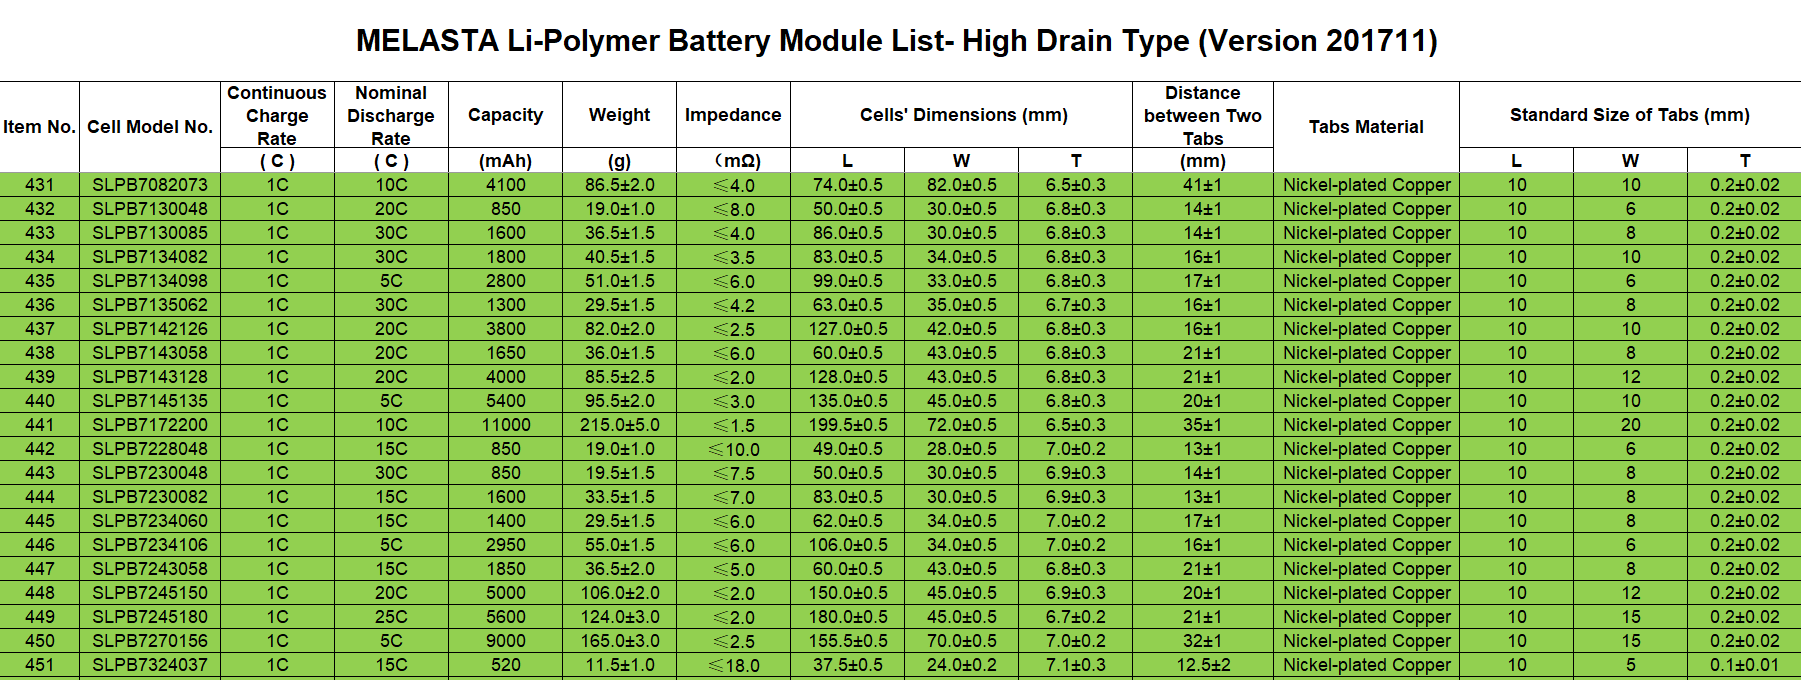
\includegraphics[width=1\linewidth]{Figures/melasta_datasheet.PNG}
	\caption{Melasta high drain pouch cell product list}
   \label{Fig:melasta_productlist}
\end{figure}

In this sheet, many important details per cell are detailed:
\begin{enumerate}
\item Continuous Charge Rate: The rate at which the cell is safely able to charge. Never exceed this charge rate or the lifespan will diminish.
\item Nominal Discharge Rate: The rate at which the cell is safely able to discharge continuously. Pulses of higher current draw is possible, but not preferred and can kill the battery. It is best to never exceed this rate.
\item Capacity: Amount of energy in the cell.
\item Weight: Total weight of the cell.
\item Impedance: Impedance is the internal resistance in the cell. This causes the heating of the cell and thus should be as low as possible.
Impedance exactly the same as resistance for DC circuits like batteries, because DC circuits do not alternate voltage/current like AC circuits do. Impedance is also affected by the frequency of this AC circuit.
\item Cell Dimension: The length, width and height of the cell.
\item Distance between Two Tabs: The distance between the two current collector tabs sticking out.
\item Standard Size of Tabs: Dimensions of both tabs.
\end{enumerate}
Like the 18650 cells, the cells get selected by allowable discharge and capacity. The capacity should range from 500 to 750\textit{Wh}. Minimal continuous discharge should be 180\textit{A}. To further reduce the list, a final criteria was added. To minimize thermal issue, it is chosen that the battery should not exceed 1.5\textit{m$\ohm$} impedance. This reduced the list to only 15 products seen in figure \ref{Fig:melasta_productlist2}.

\begin{figure} [H]
	\centering
	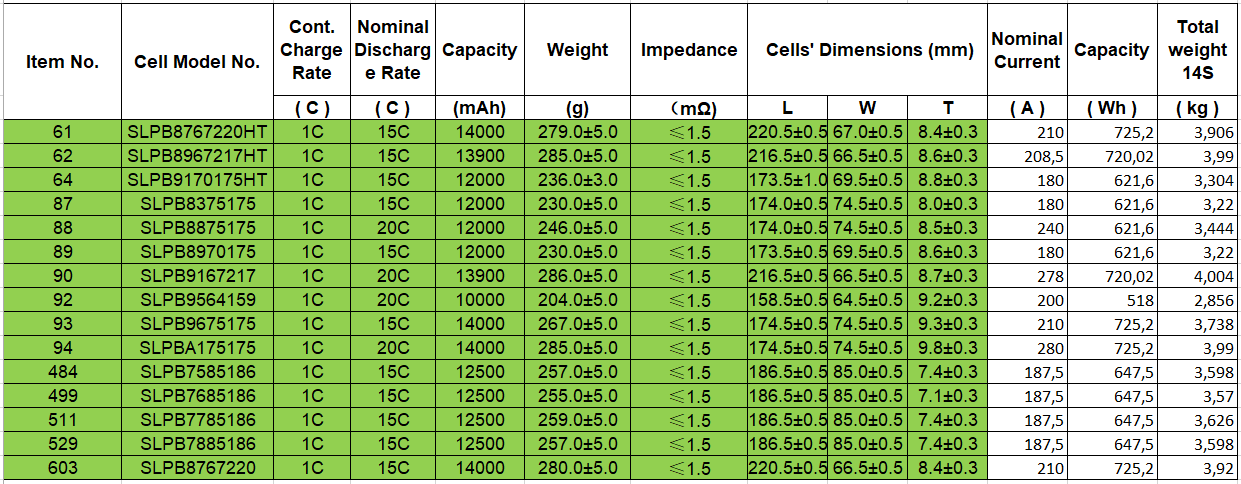
\includegraphics[width=1\linewidth]{Figures/melasta_datasheet2.PNG}
	\caption{Remaining products after criteria}
   \label{Fig:melasta_productlist2}
\end{figure}

From these 15 products, item number 87 is the lightest with enough capacity for a full 3 minute flight. Item number 87 has however only 180\textit{A} to deliver. In theory this should be fine, however this discharge should never be exceeded and it chosen to select a battery with more maximal continuous discharge. Item number 499 would then be the next option. It is the lightest with more than 180\textit{A} and enough capacity. However, finally battery 92 is chosen. It is the lightest and smallest of all, it has a 200\textit{A} continuous current draw. It does not have the required capacity of 547.22\textit{Wh} though. It is still selected because it is still close to a 3 minute cruise speed flight, and the flight will probably never actually be 3 minutes at cruise speed. The capacity is thus thought to be sufficient. Since the capacity is sufficient, and the weight and current draw is superior, item number 92 is chosen. This reduces the list to one product: The Melasta SLPB9564159. 

\begin{figure} [H]
	\centering
	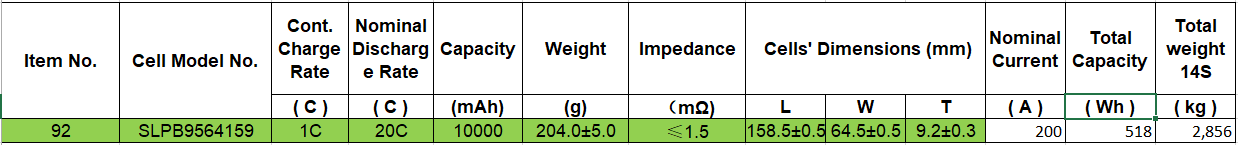
\includegraphics[width=1\linewidth]{Figures/melasta_datasheet3.PNG}
	\caption{The chosen Melasta SLPB9564159 pouch cell}
   \label{Fig:melasta_SLPB9564159}
\end{figure}

Each SLPB9564159 cell costs \euro38.77, which is in total \euro542.78 for the 14 cells.
\newpage